% Created 2020-05-06 mié 13:56
% Intended LaTeX compiler: pdflatex
\documentclass[a4paper, 12pt]{article}
\usepackage[utf8]{inputenc}
\usepackage[T1]{fontenc}
\usepackage{graphicx}
\usepackage{grffile}
\usepackage{longtable}
\usepackage{wrapfig}
\usepackage{rotating}
\usepackage[normalem]{ulem}
\usepackage{amsmath}
\usepackage{textcomp}
\usepackage{amssymb}
\usepackage{capt-of}
\usepackage{hyperref}
\usepackage{float, amsfonts, commath, mathtools}
\author{Tabaré Pérez}
\date{\today}
\title{Lecture 14 - 5: Determining the Number of Clusters}
\hypersetup{
 pdfauthor={Tabaré Pérez},
 pdftitle={Lecture 14 - 5: Determining the Number of Clusters},
 pdfkeywords={},
 pdfsubject={},
 pdfcreator={Emacs 26.3 (Org mode 9.3.6)}, 
 pdflang={English}}
\begin{document}

\maketitle
And now I would like to move to the next question we have for today is how we
can determine the number of clusters \(K\).

So let's go to this question.

Now if you remember, when I define you what clustering is, I told you you're
given points \(x\) and somebody give you number \(K\) and now your goal is to go
and find the best partitioning according to some cost.

I never told you how actually to find number \(K\). And for people who
practically use clustering algorithm, this is a real question because in most
cases, you will not be provided with a number \(K\).

So let me first start by saying that in some cases, you may intuitively know
what is the number \(K\).

So for instance, if you're teaching class at MIT, you may be given five
recitations and you need to take your whole class and divide to five recitations
based on some principle.

So in this case, maybe you think you should be getting 10 recitations, but you
have 5, you're limited by 5 and that's how you would assign the number of
clusters is given to you and you need to operate within this reality.

However, in many cases you actually
have some freedom in selecting the number \(K\).

Let's first look
at the connection between the number \(K\) and our cost function.
So what I'm going to draw you now
is like, a small graph here:


\begin{figure}[H]
\centering
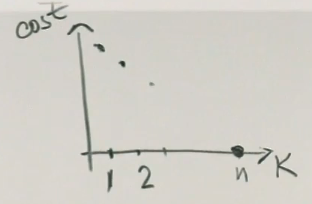
\includegraphics[width=0.5\textwidth]{./pic/u04-l14-05-fig-01.png}
\caption{\label{fig:orgcec3e1f}Cost as a function of \(K\)}
\end{figure}

So this will be number \(K\), it's our number of clusters, and this is the cost.
So the question is how does \(K\) affect the cost?

So if we put all our points in a single cluster, which means we have one
representative. Let's make it simple, talk about K-means. We have one
representative, and then we have all this end points which are closest to you.
So that's where the cost will be the highest, because now everybody, it doesn't
matter how far they're allocated, compared against one representative.

Now if you are allowed to have, let's say, two clusters, it's already better,
because now we have two representatives of at least some points, a kind local
center and will decrease the cost.

As we increase the number of clusters, we would expect that the cost would
decrease. Eventually, when every single point can be its own cluster, in this
case, the cost would be equal to \(0\).Because in this case, everybody are their
own representative, the distance is equal to \(0\).

So what do we see here that this is the relation between the cost and number of
clusters.

Now there is the question how do I know what is the right \(K\)?

And if you remember the example that I gave you about the cartoon and the image
quantization, we see this whenever we're making this choice, we are typically
driven by the application.

It's true that in this case, our cost of the partitioning becomes 0. But in the
case of image quantization, it would mean that we don't do any compression, that
every pixel stays as it is, it's represented by 24 bits, and we are not saving
anything. Our image is perfect. We're not compressing it. But you are not saving
any storage space.

So the question for many cases would be how do we have value in this case, the
compression quality and the image quality?

So let me give you some idea how we may do it if we have some task in mind.

If you're just doing it for visualization purposes, you can try with different
values of \(K\) and see if you like the picture, how it looks, if it provides
you enough insight on the data.

But in many cases, clustering when it's used as part of the machine learning
system, it can be a way to pre-process the data.

In that case, we actually do have a mechanism that enables us to select this
number \(K\).

So let's assume the following scenario:

Let's go back to what you've studied about supervised learning. You have some
supervised learning task, so you have your supervised learning task. So here you
have maybe some positives points and you have several negative points. This is
your supervised learning.

And in case of you supervised learning, you actually have very few points.

I mean, you can train your classifier, and based on this points, decides how
your separator goes.

But because you have very few points, you don't really know what is a good
boundary. Where to put the separator? Correct?

Because you have very few annotations now imagine to yourself that you also have
large number of unsupervised points for which you don't know the label \(y\),
but you know that this points belongs to this domain.

Now intuitively speaking, if you can cluster these points and understand somehow
what is the structure of these points, it may help you to better find where to
put the separator in the supervised case.

And one way to think about it, when we are generating the features, we can let's
say, run our K-means clustering and then represent every single point here not
by its cluster, because it's not good enough representation, but let's say for
by its distance to the centroid of the computed clusters.

So in addition to having the point itself, you also look how far it is located
from the centroids of all the clusters.

And now in addition to however you represented the point \(x\), you would also
add some information, which tells how geometrically it relates to all the
pre-computed clusters.

And in this case, if you do this type of representation, you can actually decide
the number \(K\) based on your development data.

You can say if I do two clusters and I do this feature representation, then my
performance on development is 75.

But if I do 20 cluster, maybe my performance on the development is going to
be 78.

And that's why I want to do this number of clusters.

So in this case, the \(K\), the granularity of partitioning that you are
getting, would be related to your performance on the final supervised learning
task.

This is one way to think about it.

So with that, we finish our unsupervised clustering part. And the last thing
that I want to say is about the word unsupervised here.

So people always feel that unsupervised means that we don't provide our system
with any knowledge, that it's just you know, you give the algorithm, the
algorithm runs and provides you the solutions.

However, even though it's unsupervised in the sense that we don't provide any
annotated points, we as people who develop those algorithms actually provide
quite a bit of indirect supervision.

We decide about which similarity measure to use. We decide about how many
clusters to give. So this is the way in clustering, where we can put our expert
knowledge and it's actually extremely important to design this similarity
functions in a way which will produce your meaningful results.

And if you're thinking about bag of words approach of representing text, these
algorithms cannot figure out which words are more semantically important than
other words.

So it would be up to you to do some weighting, so that the clustering results is
actually acceptable.

Therefore, we need to think very carefully how to do these decision choices so
that our clustering is consistent with the expectation.

And we will continue discussion about other unsupervised technique as part of
the model about generative models.
\end{document}